\documentclass{article}
\usepackage{graphicx}
\usepackage{subfigure}
\usepackage{amsmath}
\usepackage[letterpaper]{geometry}
\title{Smoothing polylines with circles}
\author{Jason Sewall}
\date{October 4, 2009}
\begin{document}
\maketitle

\section{The problem}
We have an ordered sequence $P$ of $n$ 2D points:

\begin{equation}
  \label{eq:points}
  P = \{ p_{0}, p_{1},\ldots,p_{n-2},p_{n-1}\}
\end{equation}

These points define a polyline with $n-1$ segments such as that in Fig.~\ref{fig:polyline}.  Let us assume that there are no two points adjacent in the sequence that are equal, and that there are no three adjacent points that are colinear; clearly we can eliminate of these adjacent repeated points or the central points in a colinear sequence without modifying the line's shape.

\begin{figure}[h]
  \centering
  \subfigure[\label{fig:polyline} A polyline $P$]{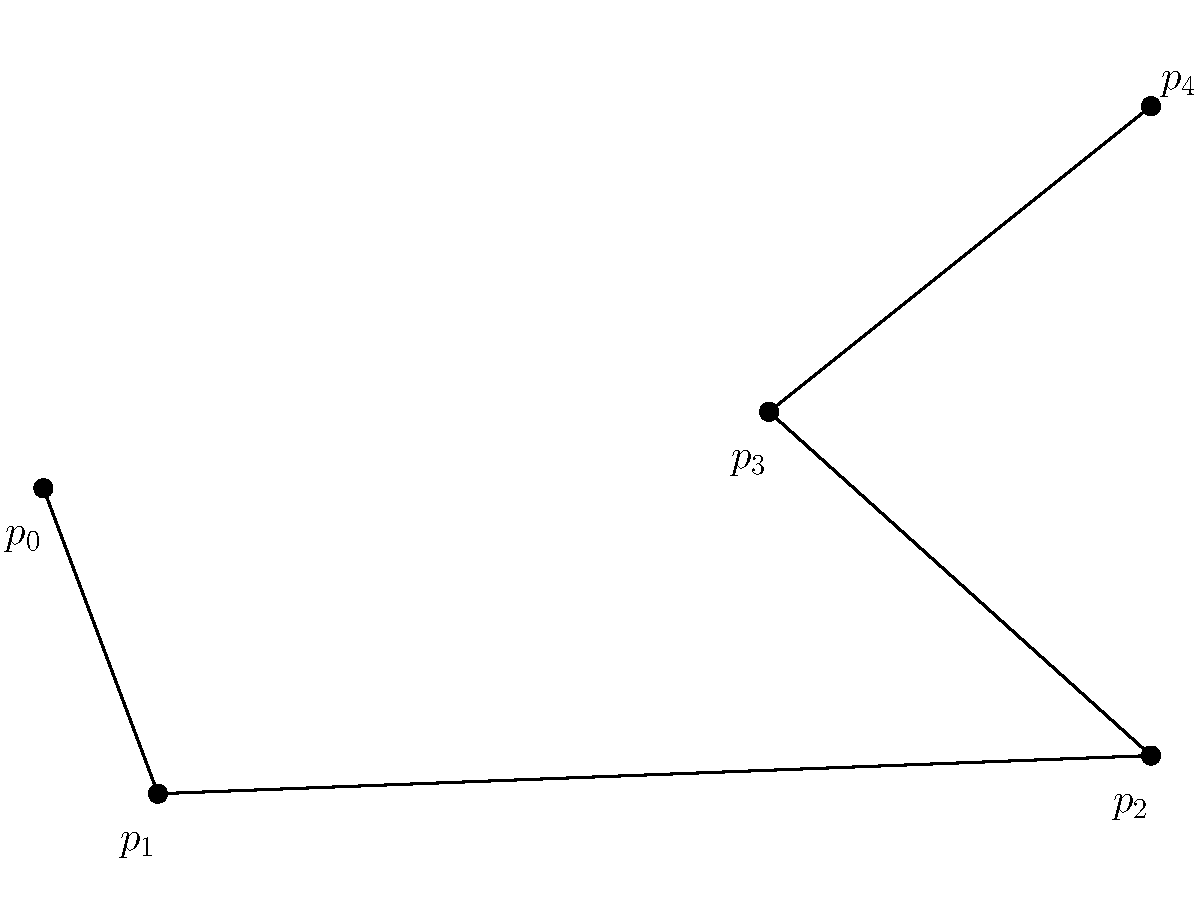
\includegraphics[width=7cm]{1}}\hfill
  \subfigure[\label{fig:smooth-polyline}A `smoothed' version of the polyline $P$]{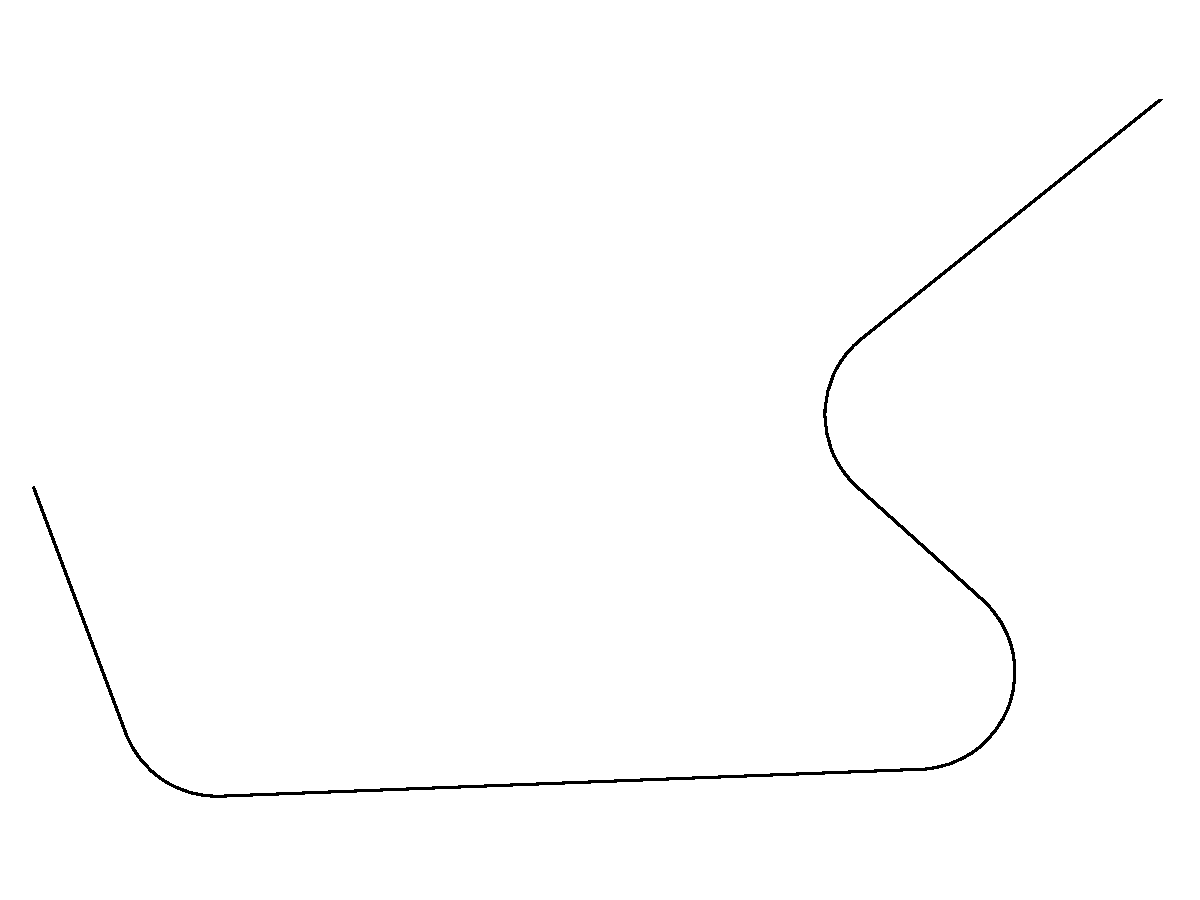
\includegraphics[width=7cm]{2}}\\
  \subfigure[\label{fig:debug-smooth-polyline}The polyline $P$ and an associated smoothed variant]{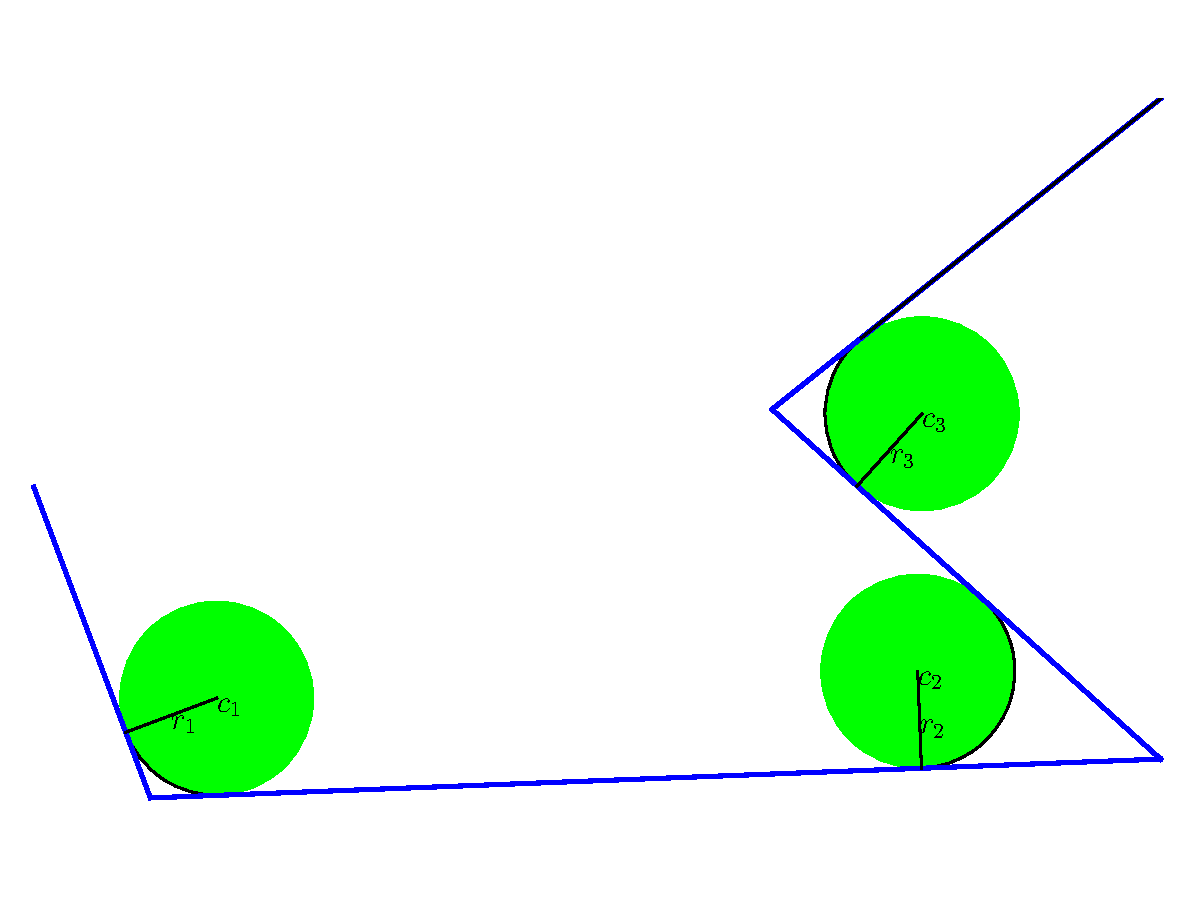
\includegraphics[width=7cm]{3}}
  \caption{Polylines}
\end{figure}

We wish to `smooth' this polyline to something like what is shown in Fig.~\ref{fig:smooth-polyline}; we shall do this by replacing the region around each interior point $p_{i}$ of $P$, with a circular arc $\mathbf{a}_{i}$.  Each $\mathbf{a}_{i}$ is defined by:

\begin{equation}
  \label{eq:circ-def}
\mathbf{a}_i=\left(
  c_{i},
  r_{i},
  \theta^{0}_{i},
  \theta^{1}_{i}
\right)
\end{equation}

Where $c_{i}$ the center, $r_{i}$ is the radius, and $\theta^{0}_{i}, \theta^{1}_{i}$ are the angular extents of the arc.  See Fig. \ref{fig:debug-smooth-polyline}; each $\mathbf{a}_{i}$ is shown.

\section{Formulation of the arcs $a_{i}$}

\subsection{Definitions}

For each interior point $p_{i}$, the associated arc $\mathbf{a}_{i}$ is determined closely associated with the triple of points:

\begin{equation}
  \label{eq:arc-triple}
  T_{i} = \left(p_{i-1}, p_{i}, p_{i+1}\right)
\end{equation}

\paragraph{Vectors}

In particular, we are interested in the derived vectors

\begin{equation}
  \label{eq:vectors}
  \begin{split}
  \mathbf{v}^{b}_{i} = p_{i-1} - p_{i}\\
  \mathbf{v}^{f}_{i} = p_{i+1} - p_{i}
  \end{split}
\end{equation}

their lengths:

\begin{equation}
  \label{eq:vector-lengths}
  \begin{split}
    L^{b}_{i} = |\mathbf{v}^{b}_{i}|\\
    L^{f}_{i} = |\mathbf{v}^{f}_{i}|
  \end{split}
\end{equation}

and the associated unit vectors:

\begin{equation}
  \label{eq:unit-vectors}
  \begin{split}
    \mathbf{n}^{b}_{i} = \frac{\mathbf{v}^{b}_{i}}{L^{b}_{i}} =\frac{\mathbf{v}^{b}_{i}}{|\mathbf{v}^{b}_{i}|}\\
    \mathbf{n}^{f}_{i} = \frac{\mathbf{v}^{f}_{i}}{L^{f}_{i}} =\frac{\mathbf{v}^{f}_{i}}{|\mathbf{v}^{f}_{i}|}
  \end{split}
\end{equation}

\paragraph{Tangent points}

The projection of $c_{i}-p_{i}$ onto $\mathbf{n}^{b}_{i}$ and onto $\mathbf{n}^{f}_{i}$ have equal length $\alpha_i$; then the tangent points of the circle on $\mathbf{v}^{b}_{i}$ and $\mathbf{v}^{b}_{i}$ are:

\begin{equation}
  \label{eq:alpha-vectors}
  \begin{split}
    (c_{i}-p_{i})\;\mathrm{proj}\; \mathbf{n}^{b}_{i} = \alpha_i\mathbf{n}^{b}_{i}\\
    (c_{i}-p_{i})\;\mathrm{proj}\; \mathbf{n}^{f}_{i} = \alpha_i\mathbf{n}^{f}_{i}
  \end{split}
\end{equation}

\paragraph{Radius vectors}

We are also interested in the (negative) radius vectors from these points to the center $c_{i}$:

\begin{equation}
  \label{eq:radius-vectors}
   \begin{split}
     \mathbf{r}^{b}_{i} = c_{i} - \left(\alpha\mathbf{n}^{b}_{i} - p_{i}\right)=\pm r_i\left( -{\mathbf{n}^{b}_{i}}_{y},  {\mathbf{n}^{b}_{i}}_{x} \right)\\
     \mathbf{r}^{f}_{i} = c_{i} - \left(\alpha\mathbf{n}^{f}_{i} - p_{i}\right)=\pm r_i\left(  {\mathbf{n}^{f}_{i}}_{y}, -{\mathbf{n}^{f}_{i}}_{x} \right)\\
   \end{split}
\end{equation}

The sign of the rightmost term in Eq.~\eqref{eq:radius-vectors} ($\pm$) is determined by the orientation of the triple $T_i$ (see Eq.~\eqref{eq:vectors}); that is to say:

\begin{equation}
  \label{eq:orientation}
  o = \mathrm{sign}\; \mathbf{n}^{b}_{i} \times \mathbf{n}^{f}_{i}
\end{equation}

See Fig.~\ref{fig:interior-point} for a visual depiction of these quantities.

\begin{figure}[h]
  \centering
  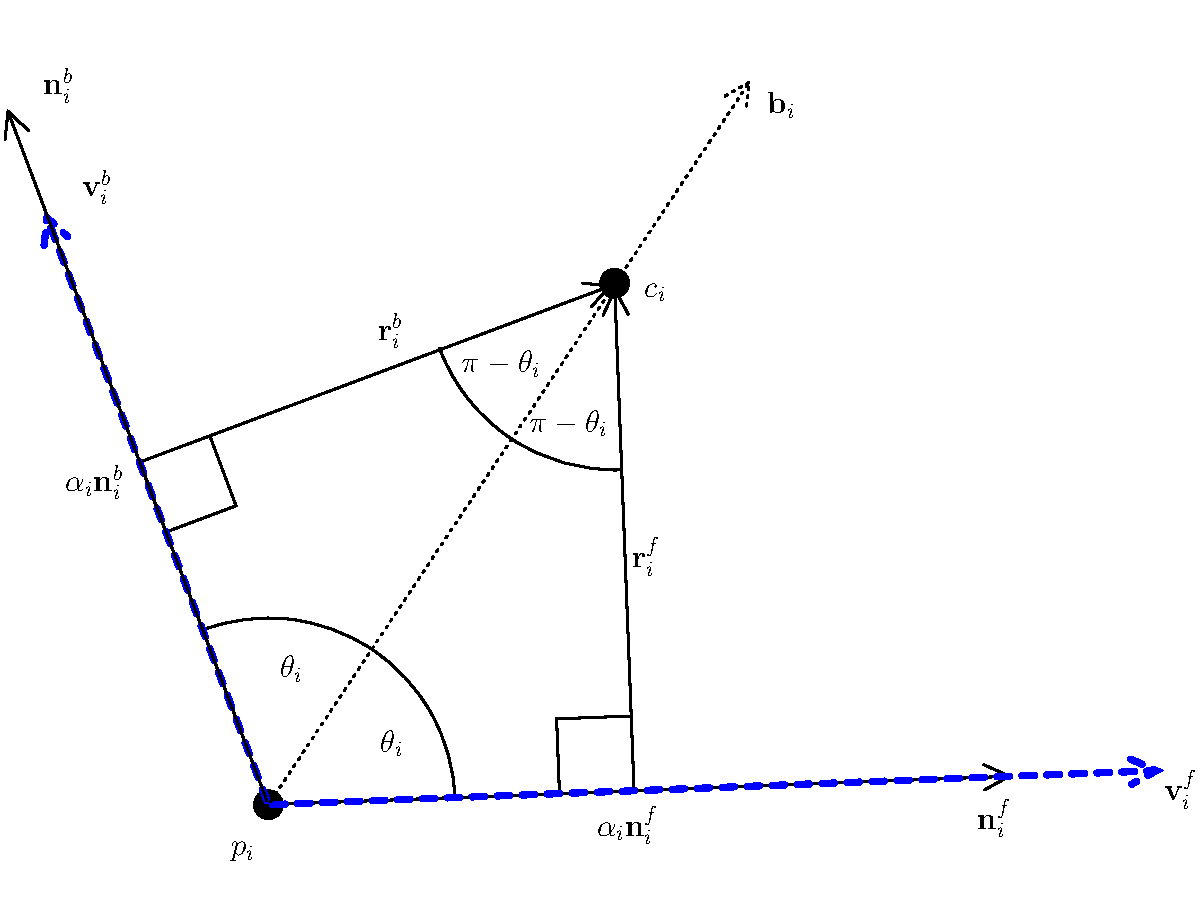
\includegraphics[width=\columnwidth]{4}
  \caption{The interior point $p_{i}$ with backward vector $\mathbf{v}^{b}_{i}$ and forward vector $\mathbf{v}^{f}_{i}$. $\mathbf{b}_{i}$ is the bisector of these vectors}
  \label{fig:interior-point}
\end{figure}

\subsection{Arc ranges}

For a given $T_i$, the arc angles $\theta^0_i$ and $\theta^{1}_{i}$; are fixed regardless of the $c_i$ or $r_{i}$:

\begin{align}
  \theta^{0}_{i} &= \arctan \frac{{\mathbf{r}^{b}_{i}}_{y}}{{\mathbf{r}^{b}_{i}}_{x}}\\
  \theta^{1}_{i} &= \arctan \frac{{\mathbf{r}^{f}_{i}}_{y}}{{\mathbf{r}^{f}_{i}}_{x}}
\end{align}

\subsection{Allowable radii}

For a given $T_{i}$, the range of suitable radii $r_{i}$ depends on $L^b_i$ and $L^f_i$; we can see in Fig.~\ref{fig:interior-point} that were $r_{i}$ to exceed some quantity, one or both of the points of tangency of the circle on the vectors may lie beyond the length(s) of the vectors --- precisely, we require:

\begin{align}
  \label{eq:alphalimit-b}
  \alpha_i &\le L^{b}_{i}\\
  \label{eq:alphalimit-f}
  \alpha_i &\le L^{f}_{i}
\end{align}

\paragraph{Lower bound}

Obviously, we know that

\begin{equation}
  \label{eq:rlow}
  r_i > 0
\end{equation}

\paragraph{Upper bound}

Now we must derive an upper bound on $r_{i}$, we based on the lengths $L^b_i$ and $L^f_i|$.  Now we can write:

\begin{equation}
  \label{eq:dotnorm}
  \mathbf{n}^{f}_{i} \cdot \mathbf{n}^{b}_{i} = \cos 2\theta_i
\end{equation}

and we are interested in

\begin{align}
  \notag
  \frac{r_i}{\alpha_{i}} &= \tan \theta_i\\
  \label{eq:tantheta}
  r_i &= \alpha_{i}\tan \theta_i
\end{align}

And we know from trigonometry that

\begin{align}
  \notag
  \tan \frac{\phi}{2} &= \frac{\sin\phi}{1+\cos\phi}\\
  \notag
  \tan \theta &= \frac{\sin 2\theta}{1+\cos 2\theta}\\
  \label{eq:tanident}
  \tan \theta &= \frac{\sqrt{1-\cos^{2} 2\theta}}{1+\cos 2\theta}
\end{align}

We can combine Eq.~\eqref{eq:tantheta} with Eq.~\eqref{eq:tanident} to get

\begin{align}
  \label{eq:radiustan}
  r_{i} &= \alpha_i\frac{\sqrt{1-\cos^{2} 2\theta_i}}{1+\cos 2\theta_i}
\end{align}

And substituting Eq.~\eqref{eq:dotnorm} into Eq.~\eqref{eq:radiustan}, we get:

\begin{align}
  \label{eq:radius-alpha}
  r_{i} &= \alpha_i\frac{\sqrt{1-\left(\mathbf{n}^f_i\cdot \mathbf{n}^b_i\right)^{2}}}{1+\mathbf{n}^f_i\cdot \mathbf{n}^b_i}
\end{align}

\end{document}

%%% Local Variables:
%%% mode: latex
%%% TeX-master: t
%%% End:
